\chapter{Clustering - KMeans Results}\label{apdx:cluster_res}
Results of clustering method that was used to train the initial wind flow prediction RNN. PCA and TSNE were applied to the $R [Rsun]$, $B [G]$ and $\alpha [deg]$ input variables of MULTI-VP. Next, a KMeans clustering was performed on the resulting representations. Only the PCA solution was used, as the KMeans applied to the TSNE of the joint inputs (Figure \ref{fig_a:tsne_joint_kmeans_2}) failed to produce a clear data division.

\begin{figure} [h]
    \caption[Visualization of the clusters obtained with the TSNE of the joint inputs.]{Visualization of the clusters obtained with the TSNE of the joint inputs. Unlike the results from the PCA on the joint inputs (Figure \ref{fig_a:kmean_joint_2d}), this method didn't produce a good division of the data as points that would be more suited in cluster 1 were assigned to cluster 0.}
    \label{fig_a:tsne_joint_kmeans_2}
    \centering
    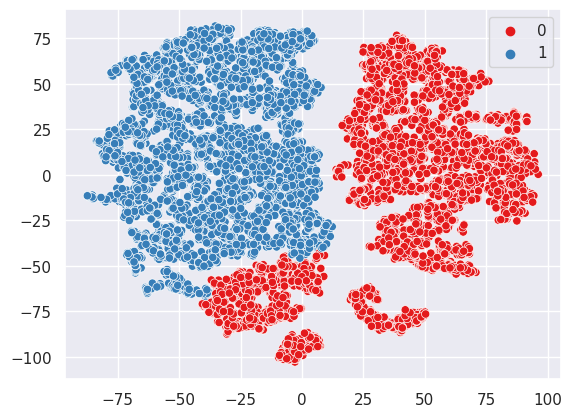
\includegraphics[width=\textwidth]{figures/tsne_joint_kmeans_2.png}
\end{figure}

\clearpage
\section{PCA Results}
\begin{figure}[h]
    \centering
    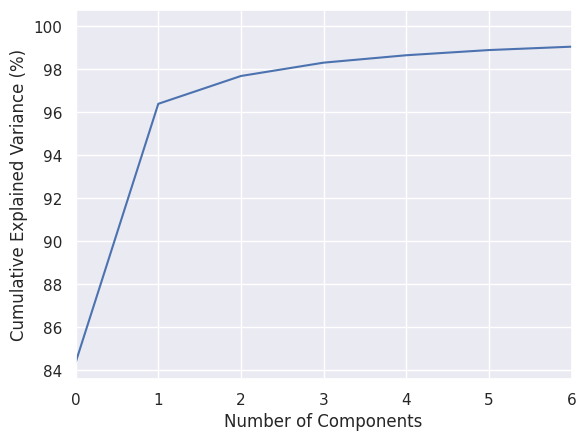
\includegraphics[width=\textwidth]{figures/join_pca_variance.png}
    \caption{Cumulative Explained Variance for the PCA of the input variables}
    \label{fig_a:cumulative_var_join}
\end{figure}

% \begin{figure}
%     \centering
%     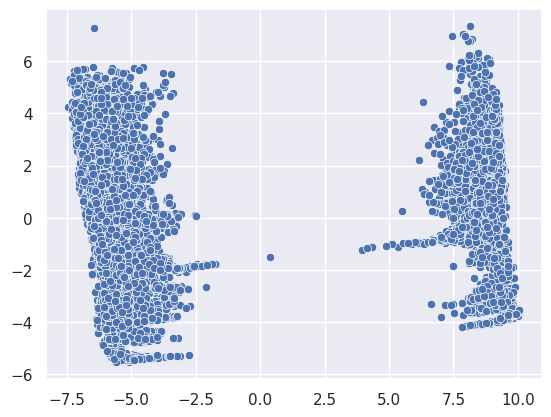
\includegraphics[width=0.8\textwidth]{figures/pca_joint_2d.png}
%     \caption{PCA of the MULTI-VP joint variables}
%     \label{fig_a:pca_joint_2d}
% \end{figure}

\begin{figure}[]
    \centering
    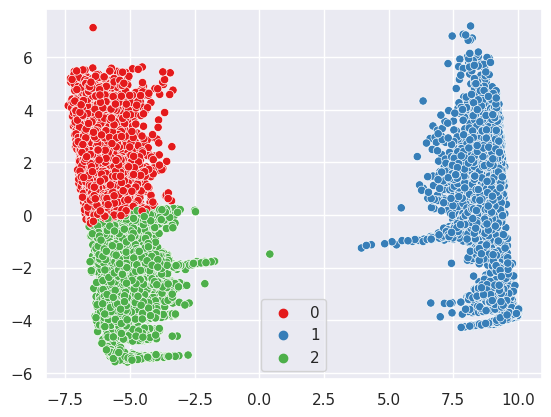
\includegraphics[width=\textwidth]{figures/kmeans_joint_pca_3.png}
    \caption{KMeans clustering of the PCA of the input variables}
    \label{fig_a:kmean_joint_2d}
\end{figure}


\begin{figure}
    \centering
    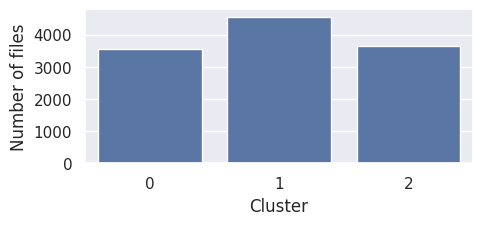
\includegraphics{figures/pca_kmeans_cluster_distr.png}
    \caption{Number of profiles per cluster}
    \label{fig_a:cluster_distr}
\end{figure}

\begin{figure}[]
    \makebox[\linewidth]{
        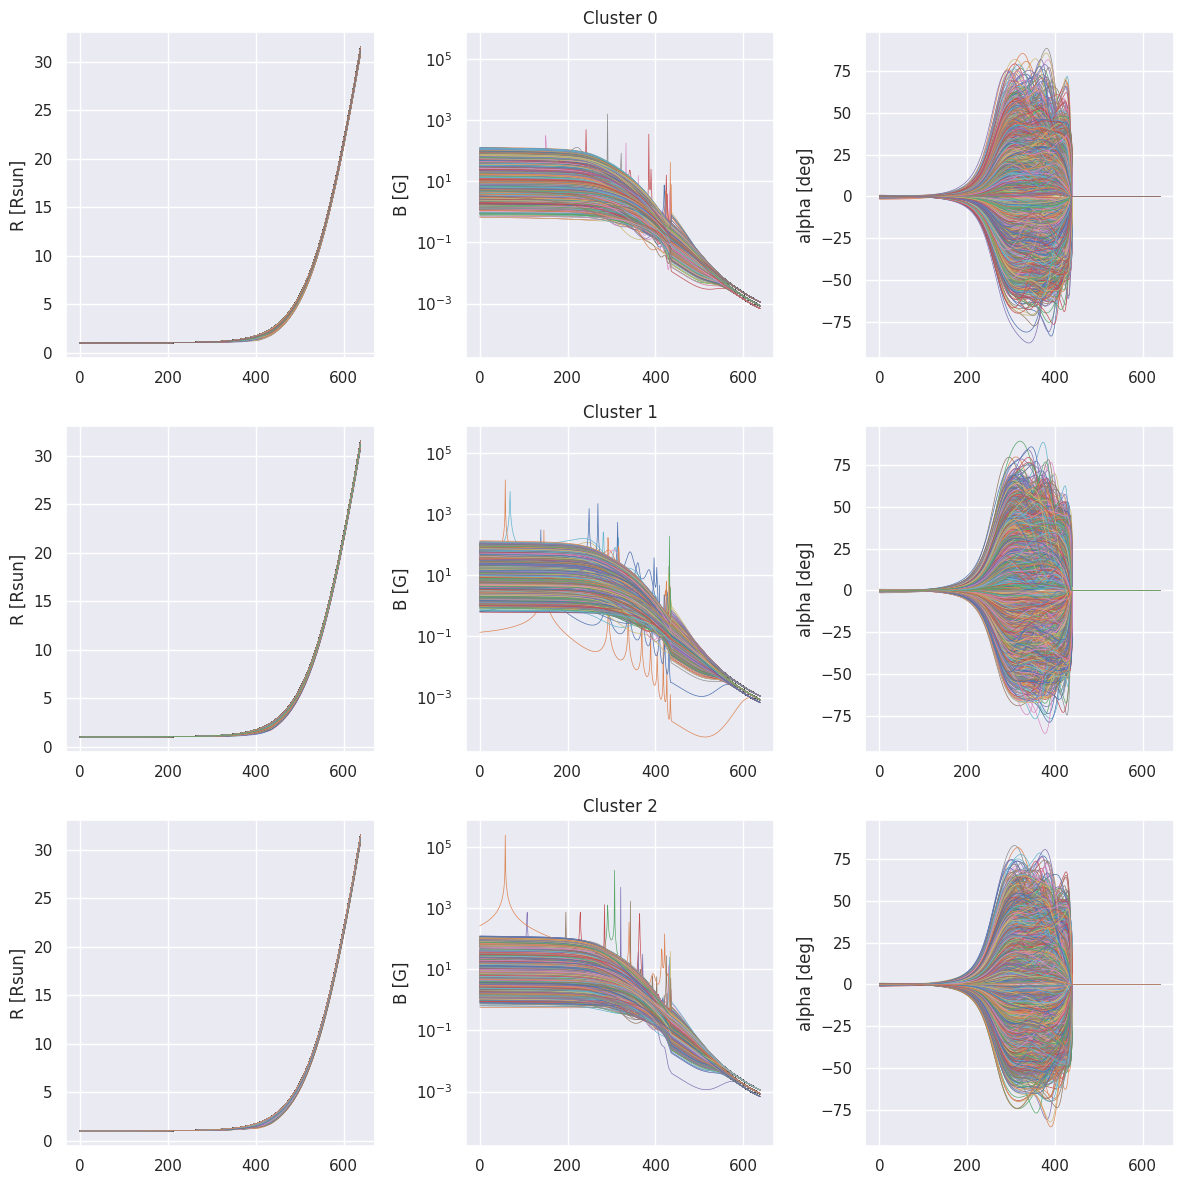
\includegraphics[width=0.9\paperwidth]{figures/line_div_kmeans_pca.png}
    }
    \caption{Data division based on the clustering results}
    \label{fig_a:real_pca_kmeans}
\end{figure}

